\documentclass[preview]{standalone}

\usepackage{amsmath}
\usepackage{amssymb}
\usepackage{stellar}
\usepackage{definitions}
\usepackage{bettelini}
\usepackage{tikz}

\begin{document}

\id{graph-prufer-code}
\genpage

\section{Cayley formula}

\begin{snippettheorem}{cayley-formula-theorem}{Cayley's formula}
    Let \(n\geq 2\). There are exactly
    \[
        n^{n-2}
    \]
    labelled trees with vertex set \(\{1,\ldots,n\}\).
\end{snippettheorem}

\begin{snippet}{cayley-formula-prufer-strategy}
    To prove Cayley's formula, one uses the Prüfer code, which assigns to each
    labelled tree on \(\{1,\ldots,n\}\) a sequence of length \(n-2\) with
    values in \(\{1,\ldots,n\}\).
\end{snippet}

\section{Prüfer code}

\begin{snippetdefinition}{prufer-deletion-sequences-definition}{Deletion sequences of a labelled tree}
    Let \(T\) be a tree with \(n\geq 2\) vertices labelled by
    \[
        1,2,\ldots,n.
    \]
    Put \(T_0=T\). We construct three sequences
    \[
        x_1,\ldots,x_{n-1},
        \qquad
        y_1,\ldots,y_{n-1},
        \qquad
        T_1,\ldots,T_{n-1}
    \]
    recursively as follows.

    At step \(i\), let \(x_i\) be the smallest leaf of \(T_{i-1}\), let
    \(y_i\) be the unique vertex adjacent to \(x_i\) in \(T_{i-1}\), and let
    \(T_i\) be the tree obtained from \(T_{i-1}\) by deleting \(x_i\) and the
    edge joining \(x_i\) to \(y_i\).
    The process stops when one vertex remains.
\end{snippetdefinition}

\begin{snippetexample}{prufer-code-computation-example}{Computing a Prüfer code}
    Consider the following labelled tree:
    \[
        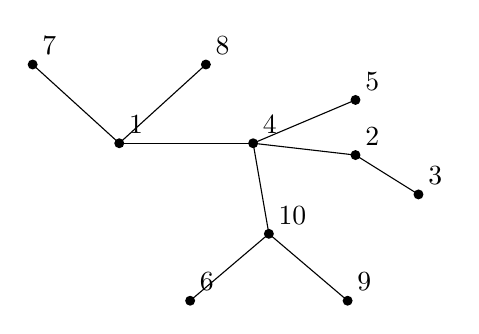
\begin{tikzpicture}[scale=1]
            \coordinate (v1) at (0,0);
            \coordinate (v7) at (-1.1,1);
            \coordinate (v8) at (1.1,1);
            \coordinate (v4) at (1.7,0);
            \coordinate (v5) at (3,0.55);
            \coordinate (v2) at (3,-0.15);
            \coordinate (v3) at (3.8,-0.65);
            \coordinate (v10) at (1.9,-1.15);
            \coordinate (v6) at (0.9,-2);
            \coordinate (v9) at (2.9,-2);

            \draw (v1)--(v7);
            \draw (v1)--(v8);
            \draw (v1)--(v4);
            \draw (v4)--(v5);
            \draw (v4)--(v2);
            \draw (v2)--(v3);
            \draw (v4)--(v10);
            \draw (v10)--(v6);
            \draw (v10)--(v9);

            \foreach \i in {1,2,3,4,5,6,7,8,9,10}{
                \fill (v\i) circle (1.8pt);
                \node[above right] at (v\i) {\(\i\)};
            }
        \end{tikzpicture}
    \]
    Applying the deletion algorithm, always deleting the leaf of smallest
    label, gives
    \[
        \begin{array}{c|ccccccccc}
            i   & 1 & 2 & 3 & 4  & 5 & 6 & 7 & 8  & 9  \\
            \hline
            x_i & 3 & 2 & 5 & 6  & 7 & 8 & 1 & 4  & 9  \\
            y_i & 2 & 4 & 4 & 10 & 1 & 1 & 4 & 10 & 10
        \end{array}
    \]
    The Prüfer code is formed by the first \(n-2\) terms of the \(y_i\)
    sequence:
    \[
        (2,4,4,10,1,1,4,10).
    \]
\end{snippetexample}

\begin{snippetproposition}{prufer-sequence-properties-proposition}{Properties of the deletion sequences}
    Let \(T\) be a labelled tree with vertex set \(\{1,\ldots,n\}\), and let
    \(x_i,y_i,T_i\) be the deletion sequences associated with \(T\). Then:
    \begin{enumerate}
        \item in the sequence \(x_1,\ldots,x_{n-1}\), the labels
        \(1,\ldots,n-1\) occur exactly once each;
        \item the pairs \((x_i,y_i)\) are exactly the endpoints of the
        \(n-1\) edges of \(T\);
        \item for every vertex \(a\), the degree of \(a\) in \(T\) equals the
        total number of occurrences of \(a\) in the combined sequences
        \[
            x_1,\ldots,x_{n-1},y_1,\ldots,y_{n-1};
        \]
        \item \(y_{n-1}=n\).
    \end{enumerate}
\end{snippetproposition}

\begin{snippetproof}{prufer-sequence-properties-proof}{prufer-sequence-properties-proposition}{Properties of the deletion sequences}
    Once a vertex is deleted, it can never appear again in the sequence
    \(x_i\). Also, as long as a tree has at least two vertices, it has at
    least two leaves. Since the algorithm always deletes the smallest leaf,
    the vertex \(n\) cannot be chosen as some \(x_i\) before the final vertex
    remains: if \(n\) were a leaf, there would still be another leaf of smaller
    label.

    Therefore the deleted vertices are precisely \(1,\ldots,n-1\), each once.
    At step \(i\), the algorithm deletes exactly the edge joining \(x_i\) to
    \(y_i\), so the pairs \((x_i,y_i)\) record all and only the edges of the
    tree.

    The degree of a vertex is the number of edges incident with it. Since the
    edges are exactly the pairs \((x_i,y_i)\), the degree of a vertex is the
    total number of times it occurs in the two sequences \(x_i\) and \(y_i\).

    Finally, since the vertex \(n\) is the last surviving vertex, the last
    deleted edge has its other endpoint equal to \(n\). Hence
    \[
        y_{n-1}=n.
    \]
\end{snippetproof}

\begin{snippetdefinition}{prufer-code-definition}{Prüfer code}
    Let \(T\) be a labelled tree with vertex set \(\{1,\ldots,n\}\), where
    \(n\geq 2\). The \emph{Prüfer code} of \(T\) is the sequence
    \[
        (y_1,y_2,\ldots,y_{n-2})\in \{1,\ldots,n\}^{n-2}
    \]
    obtained from the deletion algorithm.
\end{snippetdefinition}

\begin{snippet}{prufer-code-map}
    The Prüfer code defines a function
    \[
        \{\text{labelled trees with } n \text{ vertices}\}
        \fromto
        \{1,\ldots,n\}^{n-2}.
    \]
    Since the codomain has cardinality \(n^{n-2}\), Cayley's formula follows
    once this function is shown to be bijective.
\end{snippet}

\begin{snippetproposition}{prufer-code-reconstruction-proposition}{Reconstruction from a Prüfer code}
    Let \(n\geq 2\). Every sequence
    \[
        (y_1,\ldots,y_{n-2})\in\{1,\ldots,n\}^{n-2}
    \]
    is the Prüfer code of exactly one labelled tree with vertex set
    \(\{1,\ldots,n\}\).
\end{snippetproposition}

\begin{snippetproof}{prufer-code-reconstruction-proof}{prufer-code-reconstruction-proposition}{Reconstruction from a Prüfer code}
    Start from an arbitrary sequence
    \[
        (y_1,\ldots,y_{n-2})\in\{1,\ldots,n\}^{n-2}.
    \]
    Put \(y_{n-1}=n\). We reconstruct the sequence
    \(x_1,\ldots,x_{n-1}\), and therefore the edges of the tree.

    Define \(x_1\) to be the smallest vertex that does not occur in
    \[
        (y_1,y_2,\ldots,y_{n-1}).
    \]
    Add the edge \((x_1,y_1)\).

    Recursively, once \(x_1,\ldots,x_{i-1}\) have been defined, define
    \(x_i\) to be the smallest vertex that does not occur in
    \[
        (x_1,x_2,\ldots,x_{i-1},y_i,y_{i+1},\ldots,y_{n-1}).
    \]
    Add the edge \((x_i,y_i)\).

    This construction is deterministic, so the sequence determines at most one
    graph. It remains to show that the graph obtained is always a tree. We
    prove this by induction on \(n\).

    If \(n=2\), the Prüfer sequence is empty. We set \(y_1=2\), choose
    \(x_1=1\), and obtain the single edge joining \(1\) and \(2\), which is a
    tree.

    Let \(n>2\) and assume the statement for \(n-1\). Apply the construction to
    the given sequence, obtaining \(x_1,\ldots,x_{n-1}\) and
    \(y_1,\ldots,y_{n-1}\). Ignore the first edge \((x_1,y_1)\) and the vertex
    \(x_1\). The remaining graph has vertex set
    \[
        \{x_2,\ldots,x_{n-1},n\}
    \]
    and edge set
    \[
        \{(x_i,y_i)\mid i=2,\ldots,n-1\}.
    \]
    By the induction hypothesis, this remaining graph is a tree.

    By definition of \(x_1\), the vertex \(x_1\) does not occur among
    \(y_1,\ldots,y_{n-1}\). Thus adding \(x_1\) and the edge \((x_1,y_1)\)
    attaches \(x_1\) as a leaf. This preserves connectedness and creates no
    cycle. Hence the whole graph is a tree.
\end{snippetproof}

\begin{snippetproof}{cayley-formula-proof}{cayley-formula-theorem}{Cayley's formula}
    The Prüfer code gives a bijection between labelled trees with vertex set
    \(\{1,\ldots,n\}\) and sequences of length \(n-2\) with values in
    \(\{1,\ldots,n\}\).
    The number of such sequences is
    \[
        \underbrace{n\cdot n\cdots n}_{n-2\text{ times}}=n^{n-2}.
    \]
    Therefore the number of labelled trees with \(n\) vertices is
    \(n^{n-2}\).
\end{snippetproof}

\end{document}
